\documentclass[letter]{article}

% Fields
\def\season{2024-2025}

\usepackage{tikz}
\usetikzlibrary{calendar,shapes,positioning}

\usepackage[parfill]{parskip}

\usepackage{titling}
\usepackage{graphicx}
\setlength{\columnseprule}{1pt}
\pretitle{%
  \AddToShipoutPictureBG*{%
  \begin{tikzpicture}[remember picture,overlay]
    \node[anchor=north west,scale=1.5] at (current page.north west){%
        
\includegraphics{FIRSTLego_iconHorz_RGB}};
    \node[anchor=north east,scale=.11] at (current page.north east){%
        
\includegraphics{FIRST_SUBMERGED_Patch_Logo_RGB}};
  \end{tikzpicture}}

  \begin{center}\Large\bfseries\MakeUppercase}
\author{}
      \title{First Lego League (FLL) \\ \season{} Season Charter}
\posttitle{%
\end{center}
\vspace{-2cm}
}
\date{}

\usepackage{geometry}
\geometry{margin=0.75in}
\usepackage{fancyhdr}

\usepackage[hidelinks]{hyperref}

\pagestyle{fancy}
\usepackage{lastpage}
\fancyhf{}
\fancyhead[L]{\season{} Season FLL Charter}
\fancyhead[R]{\thepage{} of \pageref{LastPage}}
\fancypagestyle{firststyle}
{
   \fancyhf{}
   \fancyfoot[C]{\footnotesize Page \thepage\ of \pageref{LastPage}}
   \renewcommand{\headrulewidth}{0pt} % removes horizontal header line
}

% % Watermark
\usepackage{eso-pic}
% \AddToShipoutPictureFG{%
%   \begin{tikzpicture}[remember picture,overlay]
%     \node[gray,rotate=45,scale=14,opacity=0.2] at (current page.center){%
%         \textbf{DRAFT}};
%   \end{tikzpicture}}

% Calendar
\makeatletter
\tikzstyle{week list sunday}=[
% Note that we cannot extend from week list,
% the execute before day scope is cumulative
execute before day scope={%
  \ifdate{day of month=1}{\ifdate{equals=\pgfcalendarbeginiso}{}{
      % On first of month, except when first date in calendar.
      \pgfmathsetlength{\pgf@y}{\tikz@lib@cal@month@yshift}%
      \pgftransformyshift{-\pgf@y}
    }}{}%
},
execute at begin day scope={%
  % Because for TikZ Monday is 0 and Sunday is 6,
  % we can't directly use \pgfcalendercurrentweekday,
  % but instead we define \c@pgf@counta (basically) as:
  % (\pgfcalendercurrentweekday + 1) % 7
  \pgfmathsetlength\pgf@x{\tikz@lib@cal@xshift}%
  \ifnum\pgfcalendarcurrentweekday=6
  \c@pgf@counta=0
  \else
  \c@pgf@counta=\pgfcalendarcurrentweekday
  \advance\c@pgf@counta by 1
  \fi
  \pgf@x=\c@pgf@counta\pgf@x
  % Shift to the right position for the day.
  \pgftransformxshift{\pgf@x}
},
execute after day scope={
  % Week is done, shift to the next line.
  \ifdate{Saturday}{
    \pgfmathsetlength{\pgf@y}{\tikz@lib@cal@yshift}%
    \pgftransformyshift{-\pgf@y}
  }{}%
},
% This should be defined, glancing from the source code.
tikz@lib@cal@width=7
]
\makeatother

\begin{document}
\maketitle
\thispagestyle{firststyle}

\hypertarget{communication}{%
\section{Communication}\label{communication}}

E-Mail distribution list. We compile an E-Mail distribution list from
recruitement events, parent requests and the orientation meeting. If you
would like to be added to the distribution list please email the head
coach at \href{mailto:ken@bellock.net}{\nolinkurl{ken@bellock.net}} and
request to be added to the list. If you are receiving emails and wish to
be removed from the list, reply (not reply-all) to an email with
``UNSUBSCRIBE'' in the subject line of the email.

\hypertarget{coach-profiles}{%
\section{Coach/Administrator Profiles}\label{coach-profiles}}

Coaches are all parent volunteers, none are paid for their time.

\hypertarget{omms-sponsor}{%
\subsection{OMMS Administrator}\label{omms-sponsor}}

This is a parent led club, but it would not be possible without
Mrs.~Hartman! She coordinates the creation of the teams, and provides us
with a space to practice, robots, Legos, and game boards. Thank you
Mrs.~Hartman!!

\hypertarget{head-coach}{%
\subsection{Coach Bellock}\label{head-coach}}

My name is Ken Bellock, and I'll be the head coach for this season's FLL
teams. I have a B.S. in Mathematics and Physics from Penn State, and a
M.S. in Geographic Information Systems from Johns Hopkins. In the past I
worked for the space program as a contractor designing ascent aborts
scenarios for the Space Shuttle. For my current job I lead a team of
Embedded Software Engineers who automate tests on satellite systems
before we deploy them to space.

\hypertarget{coach-barcelo}{%
\subsection{Coach Barcelo}\label{coach-barcelo}}

My name is Brendan Barcelo, and this is my third season coaching FLL. This year I'll be one of your assistant coaches. I have a B.S. in Business Management and M.S. in International Business from Saint Mary's University of Minnesota. In the past I've worked for the U.S Department of State and the International Spy Museum. For my current job at U.S. Agency for International Development (USAID) I lead a team of senior technical experts advancing US foreign policy in 34 countries throughout Asia on economic growth, agriculture, energy, infrastructure, education, health, democracy and governance, elections, and gender programs.

\hypertarget{coach-fletcher}{%
\subsection{Coach Fletcher}\label{coach-fletcher}}

My name is Boyd Fletcher, I have a degree in Computer Science from Old Dominion University. I currently work for the Department of Defense and run a software and systems engineering group. I coached one of the two OMMS FLL teams in the 2023/2024 season.

\hypertarget{future-coaches}{%
\subsection{Future Coaches}\label{future-coaches}}

Coaching Help is Needed! We have several returning assistant coaches
this year, but we need more! If you are interested in helping out with
coaching please contact Coach Ken and we can talk about how you can contribute.
Any and all help will be appreciated. You do not need to know anything about coding or building with Legos to help out. We are required to have at least two coaches per team we field during competition. We especially need assistance in the instruction of public speaking and pitch presentation.

\hypertarget{meeting-schedule}{%
\section{Season Schedule}\label{meeting-schedule}}

Thursdays 6-8pm except when the school is closed and on Halloween. Usually
early after the new year we have competition (I do not know dates yet)
If we win a bracket, we move up and will have another day of
competition. Before competition we will meet on the weekends at a coach
or parents house to develop our robot game and presentation. These are
not required meetings, but are a lot of fun and very helpful for last
minute preparations for competition.

\textbf{Plan on qualifiers being held in late January, but we often do not know the exact time and location till a few weeks or a few days prior to the qualifier.}

\begin{center}
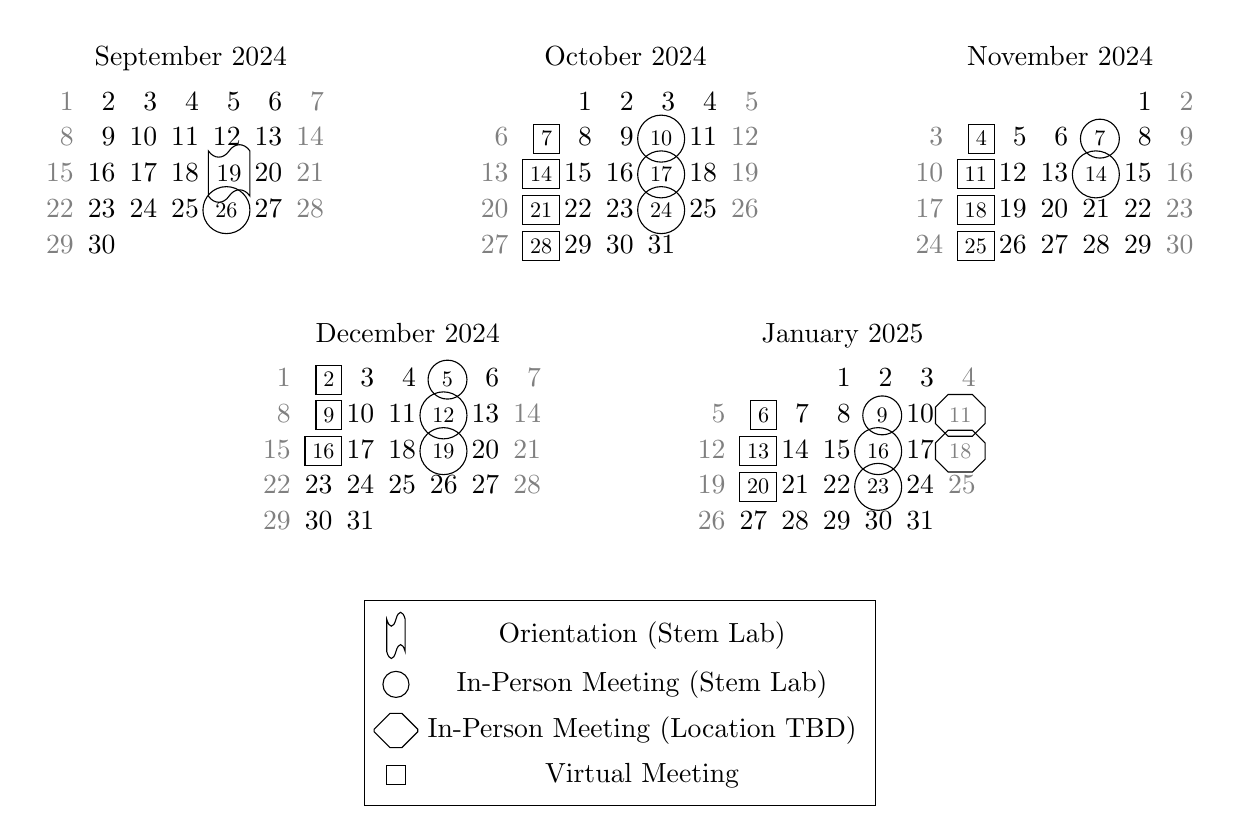
\begin{tikzpicture}[every calendar/.style = {
    month label above centered,
    month text = {\%mt \%y0},
    if={(weekend) [black!50]},
    week list sunday}]
  \matrix[column sep=5em, row sep=1em] {
    \calendar[dates=2024-09-01 to 2024-09-last]
      if (equals=2024-09-19) [nodes={tape,draw,scale=.9}]
      if (equals=2024-09-26) [nodes={circle,draw,scale=.8}]
    ; &
    \calendar[dates=2024-10-01 to 2024-10-last]
      if (equals=2024-10-07) [nodes={rectangle,draw,scale=.8}]
      if (equals=2024-10-10) [nodes={circle,draw,scale=.8}]
      if (equals=2024-10-14) [nodes={rectangle,draw,scale=.8}]
      if (equals=2024-10-17) [nodes={circle,draw,scale=.8}]
      if (equals=2024-10-21) [nodes={rectangle,draw,scale=.8}]
      if (equals=2024-10-24) [nodes={circle,draw,scale=.8}]
      if (equals=2024-10-28) [nodes={rectangle,draw,scale=.8}]
    ; &
    \calendar[dates=2024-11-01 to 2024-11-last]
      if (equals=2024-11-04) [nodes={rectangle,draw,scale=.8}]
      if (equals=2024-11-07) [nodes={circle,draw,scale=.8}]
      if (equals=2024-11-11) [nodes={rectangle,draw,scale=.8}]
      if (equals=2024-11-14) [nodes={circle,draw,scale=.8}]
      if (equals=2024-11-18) [nodes={rectangle,draw,scale=.8}]
      if (equals=2024-11-25) [nodes={rectangle,draw,scale=.8}]
    ; \\
  };
  \matrix[column sep=5em, row sep=1em,yshift=-10em] {
    \calendar[dates=2024-12-01 to 2024-12-last]
      if (equals=2024-12-02) [nodes={rectangle,draw,scale=.8}]
      if (equals=2024-12-05) [nodes={circle,draw,scale=.8}]
      if (equals=2024-12-09) [nodes={rectangle,draw,scale=.8}]
      if (equals=2024-12-12) [nodes={circle,draw,scale=.8}]
      if (equals=2024-12-16) [nodes={rectangle,draw,scale=.8}]
      if (equals=2024-12-19) [nodes={circle,draw,scale=.8}]
    ; &
    \calendar[dates=2025-01-01 to 2025-01-last]
      if (equals=2025-01-06) [nodes={rectangle,draw,scale=.8}]
      if (equals=2025-01-09) [nodes={circle,draw,scale=.8}]
      if (equals=2025-01-11) [nodes={chamfered rectangle,draw,scale=.8}]
      if (equals=2025-01-13) [nodes={rectangle,draw,scale=.8}]
      if (equals=2025-01-18) [nodes={chamfered rectangle,draw,scale=.8}]
      if (equals=2025-01-16) [nodes={circle,draw,scale=.8}]
      if (equals=2025-01-20) [nodes={rectangle,draw,scale=.8}]
      if (equals=2025-01-23) [nodes={circle,draw,scale=.8}]
    ; \\
  };
  \matrix[draw,yshift=-20em] {
      \node [tape,draw] {}; &
      \node {Orientation (Stem Lab)}; \\
      \node [circle,draw] {}; &
      \node {In-Person Meeting (Stem Lab)}; \\
      \node [chamfered rectangle,draw] {~~}; &
      \node {In-Person Meeting (Location TBD)}; \\
      \node [rectangle,draw] {}; &
      \node {Virtual Meeting}; \\
  };
\end{tikzpicture}
\end{center}

\hypertarget{game-overview}{%
\section{Game Overview}\label{game-overview}}

Students build robots with official Lego parts and program those robots to autonomously complete missions. Competition consists of the robot challenge, a core values presentation, a conversation with judges about robot design, and an innovation project presentation.  Last year we competed against over 35 thousand teams.  This is a very large and well organized international competition.

\href{https://youtu.be/c2f-Q5GGt2Q}{\textbf{Season Promotional Video:} \nolinkurl{https://youtu.be/c2f-Q5GGt2Q}}

\href{https://youtu.be/J5u-2q_K3O0}{\textbf{Robot Missions Overview:} \nolinkurl{https://youtu.be/J5u-2q_K3O0}}

\href{https://firstinspires.blob.core.windows.net/fll/challenge/2024-25/interactive-rgr/index.html}{\textbf{Official Rulebook for Robot Competition:} \nolinkurl{https://firstinspires.blob.core.windows.net/fll/challenge/2024-25/interactive-rgr/index.html}}

\href{https://firstinspires.blob.core.windows.net/fll/challenge/2024-25/fll-challenge-submerged-rubrics-color.pdf}{\textbf{Rubric for Presentations:} \nolinkurl{https://firstinspires.blob.core.windows.net/fll/challenge/2024-25/fll-challenge-submerged-rubrics-color.pdf}}

\section{Team Organization}

After the first meeting or two where everyone can get to know each other, we will organize into two competition teams and a recreational team.  The two competition teams will have 6 team members each.  The remaining students will participate on the recreational team, which allows for a less stressful and competition focused participation.  

\section{Club Rules}

\begin{enumerate}
  \item Have Fun!
  \item Students must do ALL of the work, coaches only provide guidance and training.
  \item No phones are allowed out during meetings.  You can bring them, but you cannot have them out unless messaging a parent or guardian.
  \item No headphones or earbuds.
  \item No early pickups unless cleared ahead of time.

      We work right up to the last minute.  Students who leave even a few minutes early break up team rhythm and leaves cleanup duty on teammates.

  \item Students may not leave the meeting room without permission from a coach.  No roaming of the school property is allowed.  Students must remain in the Stem Lab area.
  \item Students can bring their own laptops, but they are responsible if they are lost, stolen or broken.
  \item Water bottles and snacks are allowed.
  \item Legos, laptops and robots stay at school.  Please do not bring anything home with you unless directed by a coach.
  \item Students on competition teams must commit to the meeting schedule.

    \begin{itemize}
      \item FLL is a team sport. Missing a meeting will hurt your team just like any other team sport.
      \item If you are not sure yet if you want to commit, please keep coming to the next several meetings to help decide.
      \item A commitment should be made by early October as that is when we will create the teams that will work together until competition.
      \item If you have days you know you will miss, please let us know as far in advance as possible.
      \item If too many days are missed, a critical role on competition day cannot be guaranteed.
    \end{itemize}

  \item Respect your teammates, coaches, and the school staff.  Disrespectful behavior will result in having a parent or guardian required for attendance.  Continued disrespectful behavior will result your removal from the club.
  \item Zero-Tolerance policy on violence or threats.  If there is an issue, de-escalate and ensure a coach is observing.
\end{enumerate}

\section{Fees}

None.  The school pays the registration fees for the competition teams, provides Legos, robots, and space to practice.

\hypertarget{donations}{%
\section{Donations}\label{donations}}

\subsection{Laptops}

We are using very old laptops and students are sometimes rough on laptops.  If you have any old laptops laying around not being used, please consider donating them to the club.  Any donated laptops will be wiped clean and we will reinstall the operating system and the Lego software.

\subsection{Legos}

If you have Legos, or Lego sets you no longer need or want, we are happy to take donations.  To be used for competition they must be original Lego brand bricks and accessories.

\subsection{Team Shirts}

If you can make or design shirts and are willing to donate or assist in getting shirts for the teams, please let us know.

\subsection{Innovation Project Supplies}

As the innovation projects form, we will send out a note to parents requesting any assistance that may be needed.  In past years this has included requests for large pieces of cardboard and parents time to act as practice judges.

\section{Questions}

If you have any questions please let us know. You can email us or ask a coach
before or after meetings.

\clearpage

\section{Roster}

By signing the below, you agree that you have reviewed all of the Charter contents and agree to all the rules and conditions described above for club participation.


\newcommand*{\SignatureAndDate}[1]{%
    \par\noindent\makebox[2in]{\hrulefill} \hfill\makebox[1.5in]{\hrulefill} \hfill\makebox[1.3in]{\hrulefill}\hfill\makebox[0.25in]{\hrulefill}\hfill\makebox[0.5in]{\hrulefill}%
}%
\par\noindent\makebox[2in][c]{\textbf{Parent/Guardian (Signature)}}      \hfill\makebox[1.5in][c]{\textbf{Student Name (Printed)}} \hfill\makebox[1.3in][c]{\textbf{Emergency Contact}} \hfill\makebox[0.25in][c]{\textbf{Grade}} \hfill\makebox[0.5in][c]{\textbf{Date}}%
\SignatureAndDate{}
\SignatureAndDate{}
\SignatureAndDate{}
\SignatureAndDate{}
\SignatureAndDate{}
\SignatureAndDate{}
\SignatureAndDate{}
\SignatureAndDate{}
\SignatureAndDate{}
\SignatureAndDate{}
\SignatureAndDate{}
\SignatureAndDate{}
\SignatureAndDate{}
\SignatureAndDate{}
\SignatureAndDate{}
\SignatureAndDate{}
\SignatureAndDate{}
\SignatureAndDate{}
\SignatureAndDate{}
\SignatureAndDate{}
\SignatureAndDate{}
\SignatureAndDate{}
\SignatureAndDate{}
\SignatureAndDate{}
\SignatureAndDate{}
\SignatureAndDate{}
\SignatureAndDate{}
\SignatureAndDate{}
\SignatureAndDate{}
\SignatureAndDate{}
\SignatureAndDate{}
\SignatureAndDate{}
\SignatureAndDate{}
\SignatureAndDate{}

\end{document}

